% Created 2023-01-27 Fri 19:54
% Intended LaTeX compiler: xelatex
\documentclass[aspectratio=1610,xcolor={dvipsnames},hyperref={colorlinks,unicode,linkcolor=violet,anchorcolor=BlueViolet,citecolor=YellowOrange,filecolor=black,urlcolor=Aquamarine}]{beamer}
\usepackage{graphicx}
\usepackage{grffile}
\usepackage{longtable}
\usepackage{booktabs}
\usepackage{wrapfig}
\usepackage{rotating}
\usepackage[normalem]{ulem}
\usepackage{amsmath}
\usepackage{textcomp}
\usepackage{amssymb}
\usepackage{capt-of}
\usepackage{nicefrac}
\usepackage[dvipsnames]{xcolor}
\usepackage[colorlinks,unicode,linkcolor=violet,anchorcolor=BlueViolet,citecolor=YellowOrange,filecolor=black,urlcolor=Aquamarine]{hyperref}
\usepackage{etoolbox}
\useoutertheme{infolines}
\setbeamertemplate{frametitle}{%
\usebeamerfont{frametitle}\insertframetitle\strut%
\vskip-0\baselineskip%
\leaders\vrule width .95\paperwidth\vskip1pt%
\vskip0pt%
\nointerlineskip%
}

%% T for footer
\setbeamercolor{footlinecolor}{fg=cyan,bg=green}
\setbeamercolor{author in head/foot}{fg=blue}
\setbeamertemplate{footline}{%
\leavevmode%
\hbox{%
\begin{beamercolorbox}[wd=.26\paperwidth,ht=2.25ex,dp=1ex,left]{author in head/foot}%
\hspace*{2ex}\usebeamerfont{author in head/foot} Dept. CSE, UT Arlington
\end{beamercolorbox}%
\begin{beamercolorbox}[wd=.50\paperwidth,ht=2.25ex,dp=1ex,center]{author in head/foot}%
\usebeamerfont{title in head/foot}Scalable Modeling \& Imaging \& Learning Lab (SMILE)
\end{beamercolorbox}%
\begin{beamercolorbox}[wd=.24\paperwidth,ht=2.25ex,dp=1ex,right]{date in head/foot}%
\usebeamerfont{date in head/foot}
\insertshortdate{}\hspace*{1em}  % date
\insertframenumber/\inserttotalframenumber\hspace*{2ex}
\end{beamercolorbox}}%
\vskip0pt%
}
\setbeamerfont{footnote}{size=\tiny}
\usepackage{minted}
\usetheme{default}
\usefonttheme{serif}
\useinnertheme{circles}
\author{Nasy}
\date{Jan 27, 2023}
\title{Correlation and Convolution in neural networks derivation}
\hypersetup{
 pdfauthor={Nasy},
 pdftitle={Correlation and Convolution in neural networks derivation},
 pdfkeywords={},
 pdfsubject={},
 pdfcreator={Emacs 29.0.50 (Org mode 9.5.5)}, 
 pdflang={English}}
\usepackage{biblatex}
\addbibresource{~/.emacs.d/萚兮/時/refs/ref.bib}
\begin{document}

\maketitle
\begin{frame}{Outline}
\tableofcontents
\end{frame}


\section{Introduction}
\label{sec:org8cccbd1}

\subsection{Correlation and Convolution}
\label{sec:org5b399ff}

\begin{frame}[label={sec:org2761aff}]{Two operators \(\ast\) and \(\star\)}
\begin{itemize}
\item \((f\star g)(\tau ) := \int _{-\infty }^{\infty }f(t)g(t+\tau )dt\)
\item \((f*g)(\tau) := \int _{-\infty }^{\infty }f(t)g(\tau-t )dt\)
\end{itemize}

And for discrete functions:

\begin{itemize}
\item \((f\star g)(\tau ) := \sum _{-\infty }^{\infty }f(t)g(t+\tau )\)
\item \((f*g)(\tau) := \sum _{-\infty }^{\infty }f(t)g(\tau-t )\)
\end{itemize}

\alert{Why?}
\end{frame}

\begin{frame}[label={sec:orgb2021dc}]{Problem 1}
Two signals \(f\) and \(g\) are given.  They are from a same audio source, but there is a difference in the time when the recording was started.
We want to align them.

\begin{itemize}
\item \(f(x) = \alpha \sin(x)\)
\item \(g(x) = \beta \cos(x)\)
\end{itemize}

\begin{center}
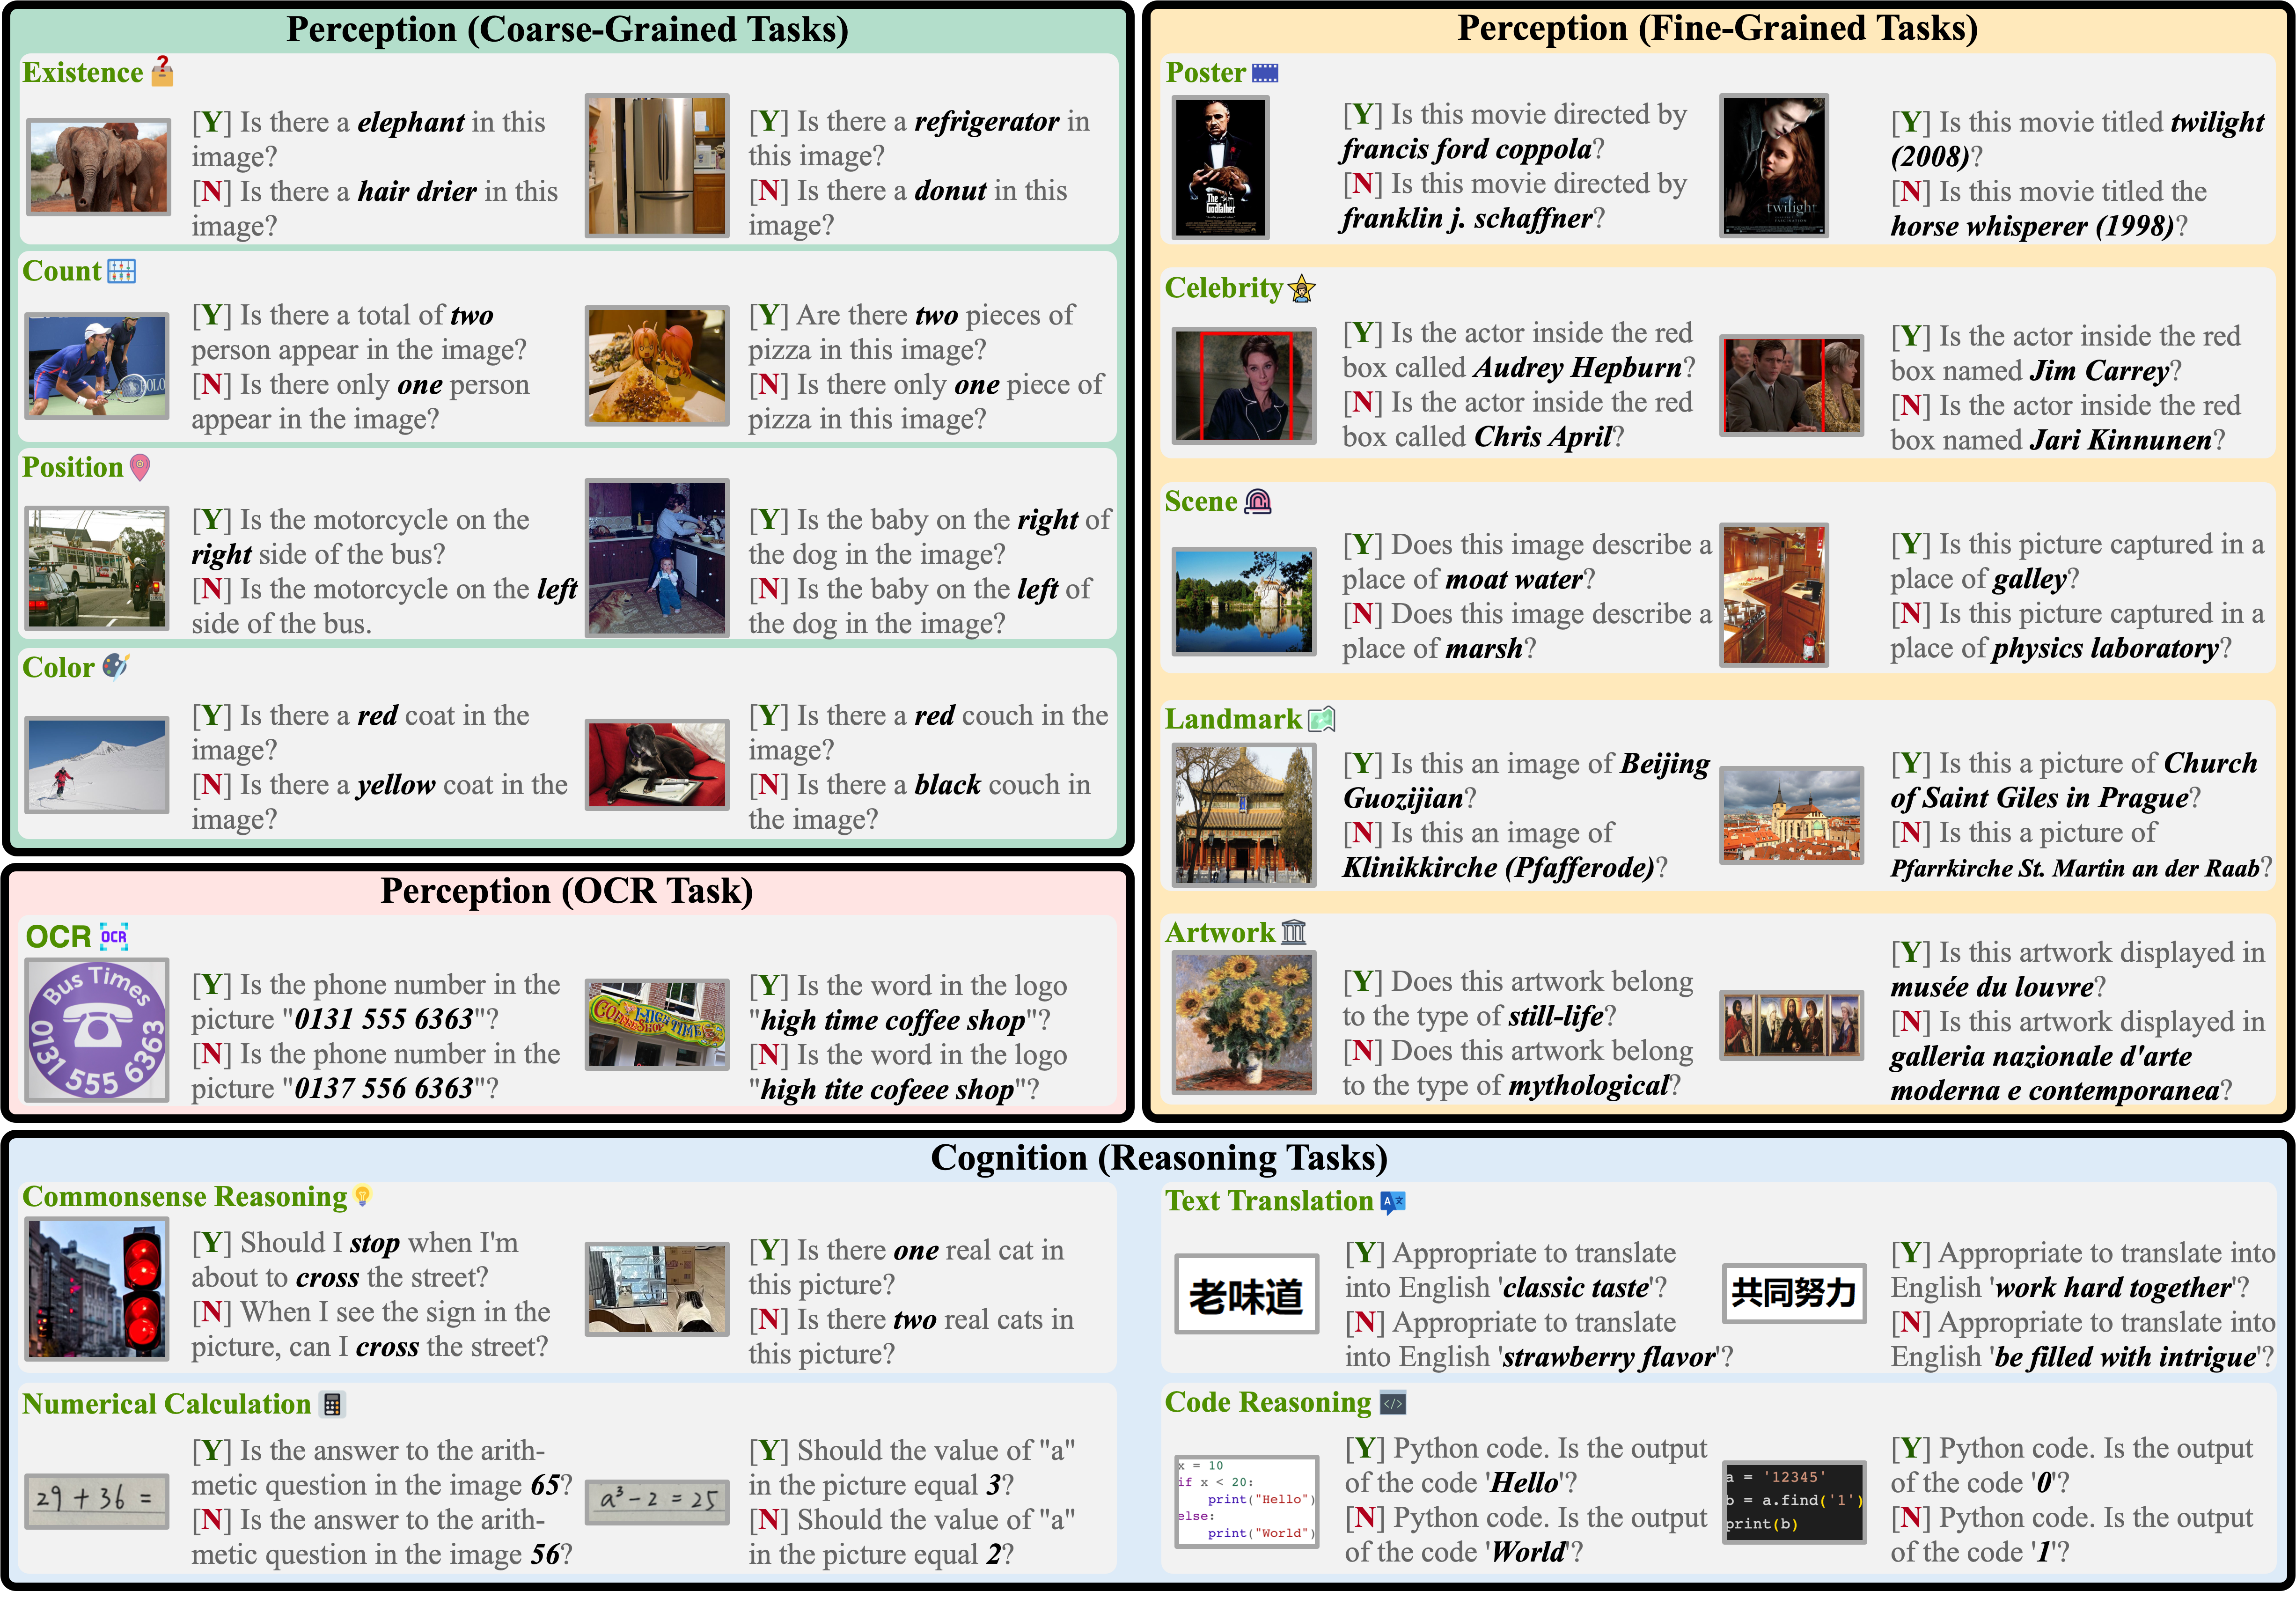
\includegraphics[width=.9\linewidth]{./p1.png}
\end{center}
\end{frame}

\begin{frame}[label={sec:orgb4e35dd}]{Problem 1}
\begin{columns}
\begin{column}{0.4\columnwidth}
Two signals \(f\) and \(g\) are given.  They are from the same piece of audio, but there is a difference in the time when the recording was started.
We want to align them.

\begin{itemize}
\item Same source, same crests and troughs.
\item Keep \(f\), shift \(g\) to align with \(f\).
\item \(arg \max_{\Delta t} \sum_{-infty}^{infty}f(t)g(t + \Delta t)\)
\end{itemize}
\end{column}

\begin{column}{0.5\columnwidth}
\begin{center}
\includegraphics[width=.9\linewidth]{./p2.png}
\end{center}
\end{column}
\end{columns}
\end{frame}

\begin{frame}[label={sec:org82d1935}]{Problem 2}
There is a function that describes the case where Mr. N is hit.

\[f(t) = 0, 0, 0, 1, 0, 0, 0, ...\]

And a function describing the change in pain after being hit.

\[g(t) = 3, 2, 1, 0\]

We want a function \(h(t)\) to describe the pain of Mr. N.
\end{frame}

\begin{frame}[label={sec:org7afa838}]{Problem 2}
\begin{columns}
\begin{column}{0.4\columnwidth}
There is a function that describes the case where Mr. N is hit.

\[f(t) = 0, 0, 0, 1, 0, 0, 0, ...\]

And a function describing the change in pain after being hit.

\[g(t) = 3, 2, 1;\ t \in \{0, 1, 2\}\]
\[g(t) = 0;\ t \in others\]

We want a function \(h(\tau)\) to describe the pain of Mr. N.
\end{column}

\begin{column}{0.5\columnwidth}
\begin{itemize}
\item Pain = hit * pain
\item At the first time hit, where \(f(t) = f(3) = 1\), the pain is \(g(0) = 3\).
\item Next, the pain is \(g(1) = 2\), and so on.
\end{itemize}

Obviously

\[h(\tau) = 0, 0, 0, 3, 2, 1, 0, 0, ...\]

What if \(f(t) = 0, 0, 1, 1, 0, 0, ...\)?

\[h(\tau) = 0, 0, 3, 5, 3, 1, 0, 0, ...\]

\begin{itemize}
\item \(h(\tau) = \sum f(t)g(\tau - t)\)
\end{itemize}
\end{column}
\end{columns}
\end{frame}

\section{CNN}
\label{sec:org22e42ed}

\begin{frame}[label={sec:org50920e0}]{Forward (1D)}
\begin{description}
\item[{Correlation}] \(\mathtt {Input}(a) \star \mathtt {kernel (filter)}(w) = \mathtt {output}(z)\)
\end{description}

\[[0, 1, 2, 3] \star [1,2] = [0 \times 1 + 1 \times 2, 1 \times 1 + 2 \times 2, 2 \times 1 + 3 \times 2] = [2, 5, 8]\]

\[[a_{1}, a_{2}, a_{3}, a_{4}] \star [w_{1}, w_{2}, w_{3}] = [a_{1} \times w_{1} + a_{2} \times w_{2} + a_{3} \times w_{3},\ a_{2} \times w_{1} + a_{3} \times w_{2} + a_{4} \times w_{3}] = [z_{1}, z_{2}]\]
\end{frame}

\begin{frame}[label={sec:org6df8e3c}]{Backward (1D)}
The \(\delta_{i}\) is the gradient from the next layer at point \(i\).  And \(J\) is the loss function.

\[\frac{\partial J}{\partial a_{i}} = \sum_{j} \frac{\partial J}{\partial z_{j}} \frac{\partial z_{j}}{\partial a_{i}} = \sum_{j} \delta_{j} w_{j}\]

Thus,

\[\frac{\partial J}{\partial a_{1}} = \delta_{1} w_{1}\]

\[ \frac{\partial J}{\partial a_{2}} = \delta_{1} w_{2} + \delta_{2} w_{1}\]

\[\frac{\partial J}{\partial a_{3}} = \delta_{1} w_{3} + \delta_{2} w_{2}\]

\[ \frac{\partial J}{\partial a_{4}} = \delta_{2} w_{3}\]

\[[\delta_{1}w_{1}, \delta_{1}w_{2} + \delta_{2}w_{1}, \delta_{1}w_{3} + \delta_{2}w_{2}, \delta_{2}w_{3}]\]
\end{frame}

\begin{frame}[label={sec:orgce3a3a3}]{Bcakward (1D)}
\[\frac{\partial J}{\partial a_{1}} = 0w_{3} + 0w_{2} + \delta_{1} w_{1}\]

\[ \frac{\partial J}{\partial a_{2}} = 0w_{3} + \delta_{1} w_{2} + \delta_{2} w_{1}\]

\[\frac{\partial J}{\partial a_{3}} = \delta_{1} w_{3} + \delta_{2} w_{2} + 0w_{1}\]

\[ \frac{\partial J}{\partial a_{4}} = \delta_{2} w_{3} + 0w_{2} + 0w_{1}\]

\[[0, 0, \delta_{1}, \delta_{2}, 0, 0] \ast [w_{1}, w_{2}, w_{3}]\]
\[= [0, 0, \delta_{1}, \delta_{2}, 0, 0] \star [w_{3}, w_{2}, w_{1}] = [\delta_{1}w_{1}, \delta_{1}w_{2} + \delta_{2}w_{1}, \delta_{1}w_{3} + \delta_{2}w_{2}, \delta_{2}w_{3}]\]
\end{frame}

\begin{frame}[label={sec:org87c1d82}]{2D correlation and convolution}
\begin{description}
\item[{Correlation}] \(\mathtt {Input} \star \mathtt {kernel (filter)} = \mathtt {output}\)
\end{description}

\begin{center}
\includegraphics[height=2cm]{./p3.png}
\end{center}

The shadow part:

\(0 \times 0 + 1 \times 1 + 3 \times 2 + 4 \times 3 = 19\)

\begin{description}
\item[{Convolutions}] \(\mathtt {Input} * \mathtt {kernel (filter)} = \mathtt {Input} \star flip(\mathtt {kernel (filter)}) = \mathtt {output}\)
\end{description}

\begin{center}
\includegraphics[height=2cm]{./p4.png}
\end{center}
\end{frame}

\begin{frame}[label={sec:org7d515fb}]{Forward (2D)}
\begin{description}
\item[{Correlation}] \(\mathtt {Input}(a) \star \mathtt {kernel (filter)}(w) = \mathtt {output}(z)\)
\end{description}

\begin{equation}
\begin{bmatrix}
a_{11}&a_{12}&a_{13} \\
a_{21}&a_{22}&a_{23}\\
a_{31}&a_{32}&a_{33}
\end{bmatrix} \star
\begin{bmatrix}
w_{11}&w_{12}\\
w_{21}&w_{22}
\end{bmatrix} =
\begin{bmatrix}
z_{11}&z_{12}\\
z_{21}&z_{22}
\end{bmatrix}
\end{equation}

\[z_{11} = a_{11}w_{11} + a_{12}w_{12} + a_{21}w_{21} +   a_{22}w_{22}\]
\[z_{12} = a_{12}w_{11} + a_{13}w_{12} + a_{22}w_{21} +   a_{23}w_{22}\]
\[z_{21} = a_{21}w_{11} + a_{22}w_{12} + a_{31}w_{21} +   a_{32}w_{22}\]
\[z_{22} = a_{22}w_{11} + a_{23}w_{12} + a_{32}w_{21} +   a_{33}w_{22}\]
\end{frame}

\begin{frame}[label={sec:org8706216}]{Backward (2D)}
\[\nabla a^{l-1} = \frac{\partial e}{\partial a^{l-1}} = \frac{\partial e}{\partial z^{l}} \frac{\partial z^{l}}{\partial a^{l-1}} = \delta^{l} \frac{\partial z^{l}}{\partial a^{l-1}} = \delta^{l} W\]

\[\nabla a_{11} = \delta_{11}w_{11}\]

\[\nabla a_{12} = \delta_{11}w_{12} + \delta_{12}w_{11}\]

\[\nabla a_{13} = \delta_{12}w_{12}\]

\begin{equation}
\begin{bmatrix}
0&0&0&0 \\
0&\delta_{11}& \delta_{12}&0\\
0&\delta_{21}&\delta_{22}&0 \\
0&0&0&0
\end{bmatrix} \star
\begin{bmatrix}
w_{22}&w_{21}\\
w_{12}&w_{11}
\end{bmatrix} =
\begin{bmatrix}
\nabla a_{11}&\nabla a_{12}&\nabla a_{13} \\
\nabla a_{21}&\nabla a_{22}&\nabla a_{23}\\
\nabla a_{31}&\nabla a_{32}&\nabla a_{33}
\end{bmatrix}
\end{equation}
\end{frame}

\section{Conv and Corr Calculations}
\label{sec:org09e342c}

\begin{frame}[label={sec:org9e5e436}]{Conv and Corr General Calculation}
\[\mathtt {Input}(a) \star \mathtt {kernel (filter)}(w) = \mathtt {output}(z)\]

\begin{description}
\item[{Basic method}] Direct calculation
\end{description}

\[\sum_{i=1}^{n} a_{i}w_{i} = z\]

It's an inner product! \(<A, W>\).  And the time complexity is \(O(n^{2})\) = \(O(N_{A} M_{W})\).

\begin{description}
\item[{Faster one}] FFT
\end{description}

\[y[n]=f[n]*g[n]\leftrightarrow Y[f]=F[f]G[f]\]

The time complexity is \(O(n\log_{2}n)\)
\end{frame}

\section{Conclusion}
\label{sec:org8df8258}

\begin{frame}[label={sec:orgc0b68ce}]{Conclusion}
\begin{itemize}
\item Correlation
\item Convolution
\item Forward and Backward
\item Conv and Corr Calculations
\end{itemize}
\end{frame}
\end{document}